\chapter{Introduction}
\label{chp:background}

\graphicspath{{images/background/}}

This thesis details the investigation of anisotropic viscosity and its use in a number of important coronal applications. The layout of the thesis is as follows. In this chapter the physics of the solar corona are introduced, including the governing magnetohydrodynamic equations and Braginskii's model of anisotropic viscosity. In chapter~\ref{chp:numerical_methods} the numerical methods underpinning the 3D magnetohydrodynamics code Lare3d (which is used to perform the numerical experiments in the remainder of this thesis) are introduced through the construction of a similar 1D hydrodynamics code. Chapter~\ref{chp:switching_model} describes the switching model, a new model of anisotropic viscosity, its implementation in Lare3d and a set of numerical experiments investigating the differences between the viscosity models when applied to a dynamically stressed magnetic null point. In chapter~\ref{chp:kink_instability}, the switching and isotropic models are compared when applied to a twisted flux rope which is initially unstable to the helical kink instability. Chapter~\ref{chp:kink_instability_straight} extends this investigation by twisting an initially straight flux tube until it becomes unstable to both the fluting and kink instabilities. In chapter~\ref{chp:null_point_khi} the switching and isotropic models are compared when applied to a magnetic null point which is twisted so rapidly that the Kelvin-Helmholtz instability is able to develop. Additionally, the chapter details the collapse of the null due to a pressure-driven asymmetry. Finally, chapter~\ref{chp:summary} presents a combined discussion of all results, beyond the separate discussions present in each chapter.

In this chapter I introduce the physics required to understand the remainder of the thesis. To give context to the work I present an overview of the layers of the Sun, including a summary of some recent developments in coronal heating. Then, I present the magnetohydrodynamic equations which are used in this thesis to model the plasma of the solar corona. Finally, I give a detailed introduction to the anisotropic nature of viscosity in a magnetised plasma and a review of modelling efforts so far.

\section{Introduction to solar physics}

\subsection{Layers of the Sun}

The stratified layers of the Sun can be considered either as part of the solar interior, located below the photosphere, or as part of the overlying solar atmosphere. The photosphere, considered the surface of the Sun, is located at a radius of $R_{\odot} = 695,508$ km.

Beneath the photosphere lie three inner regions: the core, the radiative region and the convection zone. From the centre of the Sun to a radius of approximately $0.2 R_{\odot}$ lies the engine of the Sun, the core, undergoing fusion and producing the energy that fuels dynamics in the overlying layers. The radiative region lies between the core and convection zone, up to a radius of approximately $0.71R_{\odot}$, and is the layer in which the density gradient is stable to convective motions and energy flows radially outwards via radiative transfer. At a radius of $0.71R_{\odot}$ the density gradient can no longer stably support the temperature gradient and convection becomes the dominant mechanism of energy transport. The convection zone performs two major functions: driving the solar dynamo which generates the solar magnetic field; and generating photospheric motions which provide a Poynting flux of energy into the solar corona. These photospheric motions are modelled as boundary conditions in the coronal simulations presented later.

Above (and including) the photosphere is the atmosphere of the Sun, consisting of the photosphere, chromosphere, transition region and corona. The photosphere is heated to a temperature of approximately $6000$ K and produced most of the visible light emitted from the Sun. As a result the photosphere is the only part of the Sun usually visible by the human eye (except during eclipses when both the chromosphere and corona can be seen). Just above the photosphere is the chromosphere, extending beyond the surface by $3000$--$5000$ km. The temperature ranges between $6000$ K at the photospheric boundary and $25,000$ K approaching the transition region, with a minimum of $3500$ K internally. The transition region, a shallow layer only a few $100$ km deep, lies between the chromosphere and the solar corona and across the layer the nature of the physics in the solar atmosphere changes rapidly. The primary change is in the extreme temperature difference across the layer, typically ranging from around $25,000$ K on the chromospheric side, to over $1,000,000$ K on the coronal side~\cite{priestMagnetohydrodynamicsSuna,mandriniMagneticFieldPlasma2000}. 

\begin{figure}[t]
  \centering
  \includegraphics[width=0.5\linewidth]{Traceimage.jpg}
  \mycaption{Solar coronal loops observed by the Transition Region And Coronal Explorer (TRACE), 171 Å filter.}{}%
  \label{fig:coronal_loops}
\end{figure}

The solar corona, the layer of focus for the remainder of this thesis, is the outermost region of the Sun, characterised by extremely high temperatures, low densities and a topologically complex magnetic field. With coronal plasmas reaching temperatures of $1$--$10$ MK, the corona emits predominantly in extreme ultraviolet and X-ray wavelengths, observable only by space-based instrumentation. The part of the corona visible to the human eye can typically only be seen during solar eclipses, where the corona appears to surround the Sun like a crown, hence the name. Due to the near-complete ionisation of plasma in the (low) corona, it is strongly coupled to the coronal magnetic field. Due to the low density, the plasma beta $\beta$ (a measure of the dominance of plasma versus magnetic pressures) is extremely small and dynamics in the corona are heavily dominated by magnetic forces as a result. Higher in the corona, $\beta$ can become larger~\cite{gomezPlasmaUpbetaEvolution2019}. Observationally, the corona appears inhomogeneous mainly due to the coronal plasma being mostly confined to hydromagnetic structures known as coronal loops. These are tubes of plasma contained within magnetic flux ropes, arch-like in shape with footpoints anchored in the high-$\beta$ photosphere and with lengths of $1$-$100$ Mm. Since heat flux within the corona is mostly directed along magnetic field lines, the loops are typically well insulated and are unable to homogenise differences in temperatures between neighbouring loops. The differences in temperatures, and thus densities, between loops manifests as differences in emission intensity. This allows clear observation of loops which are hotter and brighter than their neighbours (for example, in figure~\ref{fig:coronal_loops}).

The most dynamically exciting loops are those which create flares, releasing their stored magnetic energy as heat, radiation and through particle acceleration. Some flaring loops are capable of ejecting a large proportion of their mass into space as coronal mass ejections. The nanoflare theory of coronal heating posits that many small flares can collectively heat the corona to its observed temperature. This is just one theory which attempts to solve the coronal heating problem.

\subsection{Coronal heating problem}

It is not well understood why the solar corona is several magnitudes hotter than underlying layers. It is well known that the magnetic field must play a large role, and that the energy source is the turbulent, convective motions observed at the photosphere~\cite{browningMechanismsSolarCoronal1991}. However, the question of which heating mechanism or mechanisms are dominant remains broadly unanswered, although there are some certainties about the nature of these mechanisms (see reviews~\cite{demoortelRecentAdvancesCoronal2015,realeCoronalLoopsObservations2014}). Most proposed models of coronal heating involve either magnetic reconnection or dissipation of magnetohydrodynamic (MHD) waves. Although wave heating is considered less feasible by some~\cite{klimchukSolvingCoronalHeating2006a}, recent observations have generated renewed interest~\cite{hahnEvidenceWaveHeating2013,demoortelRecentAdvancesCoronal2015,mcintoshAlfvenicWavesSufficient2011,jessAlfvenWavesLower2009,depontieuChromosphericAlfvenicWaves2007}. Of the proposed reconnection-based theories, one which has been particularly successful is the nanoflare theory of coronal heating~\cite{klimchukSolvingCoronalHeating2006a}, which suggests the corona is heated by the collective sum of many small, transient heating events. 

Although there are many kinds of impulsive heating events which could constitute a nanoflare, one which has received a notable amount of attention is the process of magnetic reconnection as part of the nonlinear development of the kink instability in a coronal loop~\cite{hoodKinkInstabilitySolar1979,browningSolarCoronalHeating2003c,hoodCoronalHeatingMagnetic2009,browningHeatingCoronaNanoflares2008a}. This instability arises in a twisted magnetic flux rope when the twist exceeds a critical value, dependent on the precise magnetic configuration~\cite{hoodCoronalHeatingMagnetic2009}. The instability results in the growth of a helical kink in the rope which presses into the surrounding magnetic field, creating current sheets and typically culminating in the release of energy in one or many reconnection events. Large amounts of heat can be generated by Ohmic, viscous and shock heating as a result~\cite{barefordShockHeatingNumerical2015,hoodCoronalHeatingMagnetic2009}. It has been shown that one loop becoming unstable to the instability can trigger the eruption of neighbouring loops, causing a chain-reaction of reconnection events~\cite{hoodMHDAvalancheModel2015}. The effect of anisotropic viscosity on the kink instability is the focus of chapters~\ref{chp:kink_instability} and~\ref{chp:kink_instability_straight}.

\subsection{Dissipation mechanisms in the solar corona}

\begin{figure}[t]
  \centering
  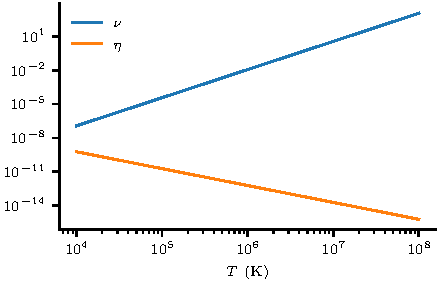
\includegraphics[width=0.5\linewidth]{visc_dep_on_temp.pdf}
  \mycaption{Dependence of non-dimensionalised viscosity $\nu$ and Spitzer resistivity $\eta$ on temperature.}{These are non-dimensionalised using typical coronal values of a magnetic field strength of $B = 5$ mT, a length of $L = 1$ Mm and a density of $\rho = 1.67 \times 10^{-12}$ kg m$^{-3}$. In the non-dimensionalisation scheme used here, the Reynolds and Lundquist numbers are the inverses of $\nu$ and $\eta$, respectively.}
  \label{fig:visc_dep_on_temp}
\end{figure}

The dominant mechanism of heat dissipation in the solar corona remains unknown, although Ohmic heating and viscous heating are two highly studied candidates. The transport parameters for viscosity $\nu$ and Spitzer resistivity $\eta$ can be derived by kinetic means as
\begin{equation}
  \label{eq:nu_and_eta}
\nu_{dim} = 10^{-17}\ T^{5/2} \text{ kg m}^{-1}\text{ s}^{-1}, \quad \eta_{dim} = 2\times 10^{9}\ T^{-3/2}\ \text{ m}^2 \text{ s}^{-1},
\end{equation}
where $T$ is the plasma temperature in Kelvin. Both expressions are taken from~\cite{braginskiiTransportProcessesPlasma1965}. Non-dimensionalising these using the scheme found in~\cite{arberStaggeredGridLagrangian2001} and typical coronal values for the Alfv\'en velocity $v_A = 3.45 \times 10^6$ m s$^{-1}$, length scale $L_0 = 1$ Mm and density $\rho_0 = 1.67 \times 10^{-12}$ kg m$^3$ give
\begin{equation}
  \label{eq:nondim_nu_and_eta}
\nu = 1.6 \times 10^{-18}\ T^{5/2} \quad \eta = 5.8 \times 10^{-4}\ T^{-3/2}.
\end{equation}
Using this non-dimensionalisation scheme the Reynolds number is given $Re = 1/\nu$ and the Lundquist number $S = 1/\eta$. Figure~\ref{fig:visc_dep_on_temp} shows the dependences of the non-dimensionalised $\nu$ and $\eta$ on temperature $T$. For a typical active region temperature of $T = 10^6$ K, $\nu \approx 10^{-3}$ and $\eta \approx 10^{-13}$.

Comparing the transport parameters for each dissipation mechanism suggests viscous heating should outperform Ohmic heating by several orders of magnitude. Indeed, many studies provide evidence to this effect~\cite{browningMechanismsSolarCoronal1991,craigViscousDissipation3D2013,craigAnisotropicViscousDissipation2009a,armstrongViscoResistiveDissipation2013,hollwegViscosityChewGoldbergerLowEquations1986a}. However, these parameters are unlikely to reflect the true degree of dissipation in the solar corona due to the influence of various effects which can enhance the effective dissipation beyond the values found via~\eqref{eq:nu_and_eta}. 

Turbulence can enhance viscosity~\cite{canutoTurbulentViscosity1988} and many mechanisms for the anomalous enhancement of resistivity have been suggested, including turbulence~\cite{cheHowAnomalousResistivity2017} and the impact of electron scattering~\cite{maEffectiveResistivityCollisionless2018}. The degree to which either dissipation mechanism is enhanced in the solar corona is difficult to estimate, however some studies have attempted to infer the effective transport parameters from observations of wave motions in coronal loops~\cite{nakariakovTRACEObservationDamped1999}, although results are disputed~\cite{klimchukCoronalSeismologyPropagation2004}. A further complication in attempting to model dissipation in the solar corona is that it is still unknown how far the collisional approximation holds~\cite{klimchukSolvingCoronalHeating2006a}.

Due to numerical diffusion present in any numerical scheme~\cite{ferzigerComputationalMethodsFluid2002}, state of the art, 3D numerical experiments are only able to probe diffusion parameters down to approximately $10^{-5}$ (non-dimensional). While this theoretically reaches the bounds of realistic viscosity, it is not close to even enhanced estimates of resistivity. Until numerical techniques and computational resources become sophisticated enough to probe realistic (enhanced or otherwise) dissipation parameters, the true nature of dissipation in the solar corona remains unclear. At best, the community can infer the importance of these and other dissipation mechanisms by constructing scaling laws for computationally feasible parameters, as is done in~\cite{craigViscousDissipation3D2013}.

\section{MHD Equations}

\subsection{The Navier-Stokes equations}

The Navier-Stokes equations are a set of partial differential equations (PDEs) which model the dynamics of a fluid through conservation of mass, momentum and energy. Generally, the equations are derived by considering conservation of the relevant quantity in a small parcel of fluid that moves with the flow. Such a derivation may be found in, for example~\cite{andersonComputationalFluidDynamics1995}. In the following description of the equations, use is made of the material derivative
\begin{equation}
  \label{eq:material_derivative}
  \frac{D}{Dt} \equiv \frac{\partial}{\partial t} + (\vec{u} \cdot \nabla)
\end{equation}
which describes the change in a quantity as it moves with flow at a velocity $\vec{u}$.

Modelling conservation of mass, the continuity equation describes the change in density $\rho$ due to the compression or dilation of the flow,
\begin{equation}
\frac{D\rho}{Dt} = - \rho \vec{\nabla} \cdot \vec{u}.
\label{eq:ns_continuity}
\end{equation}
The momentum equation is an application of Newton's second law and models the conservation of momentum in a fluid with a scalar thermal pressure $p$ and viscous stress tensor $\ten{\sigma}$,
\begin{equation}
\rho\frac{D\vec{u}}{Dt} = -\vec{\nabla} p + \vec{\nabla} \cdot \ten{\sigma}.
\label{eq:ns_momentum}
\end{equation}
The energy equation is given as
\begin{equation}
\rho\frac{D\varepsilon}{Dt} = -p \vec{\nabla} \cdot \vec{u} + \ten{\sigma} : \vec{\nabla}\vec{u},
\label{eq:ns_energy}
\end{equation}
and describes the change in internal thermal energy due to work done by pressure and viscous heating. Here, the double dot product (or tensor double contraction) is defined as $\ten{A}:\ten{B} = A_{ji} B_{ij}$ for arbitrary tensors $\ten{A}$ and $\ten{B}$. This system of equations must be closed by an additional equation of state. As presented later, the ideal equation of state is sufficient, for the purposes of describing coronal plasma.

While the Navier-Stokes equations adequately describe many fluids, conducting fluids like ionised plasmas and liquid metals couple with local magnetic fields and require an extension to the governing equations. The result are the equations of magnetohydrodynamics.

\subsection{Magnetohydrodynamics and the induction equation}

Magnetohydrodynamics (MHD) describes electrically conducting fluids, that is fluids which interact with electromagnetic fields. Typical examples of such fluids are ionised plasmas and molten metals, the investigation of the latter being key to the understanding of the Earth's molten outer core and its associated magnetic dynamo. Both small-scale laboratory plasmas, such as those found in current fusion devices, and large-scale astrophysical plasmas, such as those in the interstellar medium, can be effectively modelled using the MHD equations. While these equations have a large range of applicability, they are limited to systems with dynamics at length scales much larger than the ion skin depth or Larmor radius, and time scales much longer than the ion gyration time. For systems where the length or time scales are too small to be described by MHD, a kinetic approach using, for example, the Vlasov or Boltzmann equations is more appropriate. The ideal MHD equations can be recovered from the Boltzmann equation by taking appropriate moments~\cite{boydPhysicsPlasmas2003}.

The MHD equations are a synthesis of the Navier-Stokes equations of fluid dynamics and Maxwell's equations of electromagnetism. The latter set of equations describes the generation of an electric field $\vec{E}$ by a charge density $\rho_c$ through Gauss's law,
\begin{equation}
  \label{eq:gauss_law}
 \nabla \cdot \vec {E} ={\frac {\rho_c }{\varepsilon _{0}}},
\end{equation}
the non-existence of monopoles in the magnetic field $\vec{B}$,
\begin{equation}
  \label{eq:gauss_law_for_magnetism}
  \nabla \cdot \vec {B} =0,
\end{equation}
the generation of electric fields due to changes in the magnetic field in time $t$ through the Maxwell-Faraday equation,
\begin{equation}
  \label{eq:maxwell_faraday}
 \nabla \times \vec {E} =-{\frac {\partial \vec {B} }{\partial t}},
\end{equation}
and the generation of magnetic fields due to currents $\vec{\jmath}$ and changing electric fields through Ampère's law,
\begin{equation}
  \label{eq:ampere_law}
 \nabla \times \vec {B} =\mu _{0}\left(\vec {\jmath} +\varepsilon _{0}{\frac {\partial \vec {E} }{\partial t}}\right).
\end{equation}
Written in SI units, these equations use the permittivity $\varepsilon_{0}$ and permeability $\mu_0$ of free space.

Many conducting fluids can be considered electrically neutral, that is on the timescale of fluid motion the charges within the fluid are able to quickly redistribute to nullify any electric forces. This is true for coronal plasmas where the electrons, being much lighter than the ions, are free to quickly redistribute imbalances in charge density. This allows Gauss's law to be entirely neglected. The displacement current, the last term in Ampère's law, can also be neglected using the assumption that fluid motions are non-relativistic, that is the typical fluid velocity is much less than the speed of light, $c$~\cite{priestMagnetohydrodynamicsSuna}.

In order to couple the fluid motion to the electromagnetic fields, a constitutive Ohm's law is also included which describes the generation of currents in response to electric fields. This eventually allows the complete elimination of $\vec{E}$ from the governing equations. In a fluid's rest frame, the current response to an electric field $\vec{E}'$ is
\begin{equation}
  \label{eq:rest_frame_ohms_law}
  \vec{\jmath} = \sigma \vec{E}',
\end{equation}
where $\sigma$ is the (finite) conductivity of the fluid. The Lorentz transformation to the frame where the fluid is moving at velocity $\vec{u}$ is
\begin{equation}
  \label{eq:resistive_ohms_law}
  {\vec {E}}+{\vec{u}}\times {\vec {B}}=\eta{\vec {\jmath}},
\end{equation}
where the conductivity has been rewritten as the resistivity $\eta = 1/\sigma$. In the case of perfect conductivity, Ohm's law is written
\begin{equation}
  \label{eq:ideal_ohms_law}
  {\vec {E}}+{\vec{u}}\times {\vec {B}}=0.
\end{equation}
Additional non-ideal physics like ambipolar diffusion and the Hall effect can be modelled through additional terms in Ohm's law. However, in the solar corona these effects are small compared to resistivity and are neglected here~\cite{priestMagnetohydrodynamicsSuna}.

Combining the remaining parts of Ampère's law, the Maxwell-Faraday equation, and the resistive Ohm's law results in the induction equation,
\begin{equation}
  \label{eq:nonsimple_induction_equation}
{\frac {\partial \vec {B} }{\partial t}} = \nabla \times (\vec{u} \times \vec{B}) - \nabla \times (\eta/\mu_0 \nabla \times \vec{B}),
\end{equation}
which, in the case of uniform resistivity, may be written
\begin{equation}
  \label{eq:induction_equation}
{\frac {\partial \vec {B} }{\partial t}} = \nabla \times (\vec{u} \times \vec{B}) + \frac{\eta}{\mu_0}\nabla^2 \vec{B}.
\end{equation}
This equation essentially describes the advection and generation of a magnetic field due to fluid motions and the diffusion of the field due to resistivity. The magnetic field must still satisfy the solenoidal constraint $\nabla \cdot \vec{B} = 0$.

In order to describe the effect of the magnetic field on the fluid, additional terms must be added to the momentum~\eqref{eq:ns_momentum} and energy~\eqref{eq:ns_energy} equations. The Lorentz force describes the force exerted by the magnetic field on the fluid and is given by
\begin{equation}
  \label{eq:lorentz_force}
\vec{\jmath} \times \vec{B}.
\end{equation}
When the fluid is resistive, the dissipation of currents can heat the fluid through a process called Joule or Ohmic heating. This is modelled in the energy equation by the term
\begin{equation}
\mu_0 \eta | \vec{\jmath} |^2.
\end{equation}

\subsection{The non-dimensionalised MHD equations}

\label{sec:mhd_equations}

Combining the fluid equations~\eqref{eq:ns_continuity}--\eqref{eq:ns_energy} and the induction equation~\eqref{eq:induction_equation}, the full set of MHD equations can be written in their non-dimensionalised form
\begin{gather}
%\begin{equation}
\label{eq:mhda}
\frac{D\rho}{Dt} = - \rho \vec{\nabla} \cdot \vec{u},\\
%\end{equation}
%\begin{equation}
\rho\frac{D\vec{u}}{Dt} = -\vec{\nabla} p + \vec{\jmath} \times \vec{B} + \vec{\nabla} \cdot \ten{\sigma},\\
%\end{equation}
%\begin{equation}
\frac{D\vec{B}}{Dt} = (\vec{B} \cdot \vec{\nabla})\vec{u} - (\vec{\nabla} \cdot \vec{u})\vec{B} + \eta \nabla^2 \vec{B},\\
%\end{equation}
%\begin{equation}
\rho\frac{D\varepsilon}{Dt} = -p \vec{\nabla} \cdot \vec{u} + {Q}_{\nu} + {Q}_{\eta},%\\
\label{eq:energy}
%\end{equation}
\end{gather}
where $\eta = 1/S$ is now the non-dimensionalised resistivity, equivalent
to the inverse of the Lundquist number $S$. This notation is used throughout the remainder of this thesis. The system is closed by the inclusion of the equation of state for an ideal gas
\begin{equation}
\varepsilon = \frac{p}{\rho(\gamma - 1)},
\end{equation}
where the specific heat ratio is given by $\gamma = 5/3$. The
  terms ${Q}_{\nu} = \ten{\sigma} : \vec{\nabla}\vec{u}$ and
  ${Q}_{\eta} = \eta | \vec{\jmath} |^2$ are viscous heating and Ohmic heating, respectively.

The non-dimensionalisation scheme is identical to that used in the code Lare3d~\cite{arberStaggeredGridLagrangian2001}, where a typical magnetic field strength $B_0$, density $\rho_0$ and length scale $L_0$ are chosen and the other variables non-dimensionalised appropriately. Velocity and time are
non-dimensionalised using the Alfv\'en speed $u_A = B_0 / \sqrt{\rho_0
  \mu_0}$ and Alfv\'en crossing time $t_A = L_0/u_A$,
respectively. Temperature is non-dimensionalised via $T_0 = u_A^2
\bar{m} / k_B$, where $k_B$ is the Boltzmann constant and $\bar{m}$ is
the average mass of ions, here taken to be $\bar{m} = 1.2m_p$ (a mass
typical for the solar corona) where $m_p$ is the proton mass. Dimensional quantities can be recovered by multiplying the non-dimensional variables by their respective reference value (e.g. $\vec{B}_{\dim} = B_0 \vec{B}$). All further reference to variables will be to their non-dimensionalised values, unless stated otherwise.

\section{Anisotropic Viscosity}

Viscosity plays an important part generally in astrophysical fluid dynamics. Recent studies have demonstrated the importance of anisotropic viscosity in coronal heating in investigations of three-dimensional (3D) null points~\cite{craigViscousDissipation3D2013}, current sheet merging~\cite{armstrongViscoResistiveDissipation2013} and flux pile-up~\cite{litvinenkoViscousEnergyDissipation2005}. There is further evidence of the importance of anisotropic viscosity in other astrophysical applications including the intracluster medium~\cite{zuhoneEffectAnisotropicViscosity2014, parrishEffectsAnisotropicViscosity2012a} and the solar wind~\cite{baleMagneticFluctuationPower2009}. In other solar applications, viscosity has a role to play in the damping of coronal instabilities~\cite{howsonEffectsResistivityViscosity2017} and waves~\cite{vranjesViscosityEffectsWaves2014, erdelyiResonantAbsorptionAlfven1995a, rudermanSlowSurfaceWave2000a}, though not all these cases have been fully explored using an anisotropic model of viscosity.

\subsection{Viscosity}

Physically, viscosity is the internal friction of a fluid arising due to interactions (typically collisions) between the particles making up the fluid. Within the context of MHD, viscosity provides two functions. The first is momentum transport, included in the momentum equation as the divergence of the viscous stress tensor $\ten{\sigma}$, written using Einstein notation as
\begin{equation}
  \label{eq:viscous_momenum_transport}
  (\nabla \cdot \ten{\sigma})_j = \frac{\partial \sigma_{ij}}{\partial x_i}.
\end{equation}

In three dimensions, the nine components of $\ten{\sigma}$ quantify the flux of each component of momentum in each direction of motion as a result of viscous diffusion. For example, the $\sigma_{xy}$ component gives the flow of $x$-momentum in the $y$-direction. Due to symmetry arising from viscosity conserving angular momentum, the tensor is symmetric, so the component $\sigma_{xy}$ also quantifies the flux of $y$-momentum in the $x$-direction. Beyond the requirement of conservation of angular momentum, it is also assumed that Stokes' hypothesis holds, that is bulk viscosity is zero and viscosity does not act under uniform compression or expansion of the fluid. This requires the viscous stress tensor to be additionally trace-free,
\begin{equation}
  \label{eq:trace_free_tensor}
  \text{tr}(\ten{\sigma}) = 0.
\end{equation}
Due to the viscous stress tensor being trace-free and symmetric, the number of independent components reduces from nine to five.

The second function of viscosity is to convert kinetic into thermal energy through work done by local deformations. This is encoded in a term in the energy equation of the MHD equations of the form
\begin{equation}
  \label{eq:viscous_heat_generation}
  \ten{\sigma} : \nabla \vec{u} = \sigma_{ij} \frac{\partial u_i}{\partial x_j},
\end{equation}
and may also be written using the rate of strain tensor $\ten{W}$ as
\begin{equation}
  \label{eq:viscous_heat_generation2}
  \ten{\sigma} : \nabla \vec{u} = \frac{1}{2} \ten{\sigma} : \ten{W},
\end{equation}
where
\begin{equation}
  \label{eq:rate_of_strain}
  \ten{W} = \nabla\vec{u} + (\nabla\vec{u})^T - \tfrac{2}{3}(\nabla \cdot \vec{u})\ten{I}.
\end{equation}
The tensor $\ten{W}$ quantifies the rate at which a parcel of fluid undergoes a deformation and is symmetric and trace-free by construction.

Many fluids encountered in nature are Newtonian fluids, that is the viscous stress arising from any deformation of the fluid is directly proportional to the rate of strain of the deformation,
\begin{equation}
  \label{eq:isotropic_viscous_tensor}
  \ten{\sigma} = \nu \ten{W},
\end{equation}
where $\nu$ is the viscous transport parameter, generally referred to as the viscosity. However, in a magnetised plasma the nature of particle collisions is distinctly different from those in a non-conducting fluid and the nature of viscosity different as a result.

\subsection{Viscosity in a magnetised plasma}

\label{sec:visc_in_magnetised_plasma}

In a Newtonian fluid, the motion of a single particle travelling with typical thermal velocity $v$ and colliding with other particles in a typical collision time $\tau$ will appear as a number of broken, straight lines, each of approximate length $l = v\tau$, where $l$ is the mean free path. These motions have no preferred direction resulting in an isotropic transfer of momentum. In contrast, in a plasma made up of charged particles with charge $e$ and mass $m$, threaded by a magnetic field of strength $B$, the particles follow helical paths of approximate radius $r = v/\omega$, where $\omega = eB/m$ is the cyclotron frequency. After a time $\tau$, a typical particle will undergo a collision and its path will describe a new helix. The total resultant motion depends on the strength of the magnetic field. In the presence of a weak field, the radius of the helix may be much larger than the mean free path or in terms of the cyclotron frequency, $\omega \tau \ll 1$. As a result, the path between collisions will be close to straight and the total path will resemble that of the motion without a magnetic field. In the presence of a strong field, $\omega \tau \gg 1$ and a typical particle will be able to wind around the field a number of times, travelling a distance $l$ along the field, before colliding. As a result the transport of momentum is strongly anisotropic to the extent that it is unaffected in the direction of the field, but strongly reduced in the transverse direction.

A characteristic coronal value of $\omega \tau$ can be calculated using expressions found in Braginskii~\cite{braginskiiTransportProcessesPlasma1965}. The collision time can be written in SI units as
\begin{equation}
  \label{eq:collision_time}
  \tau = 0.82 \times 10^{-6} \frac{T^{3/2}}{n} \text{ s},
\end{equation}
where $n$ is the number density. The cyclotron frequency is written as
\begin{equation}
  \label{eq:cyclotron_frequency}
  \omega = 0.96\times10^8 B \text{ s}^{-1},
\end{equation}
where the Coloumb logarithm has been taken to be 22, and the mass fraction, the ratio of ion to proton mass, $m_f = m_i/m_p$ has been taken to be a typical solar value of $1.2$. A solar active region has typical temperatures of around $2\times 10^6$ K and number densities of $n = 3 \times 10^3\text{ m}^{-3}$, giving $\tau = 0.773$ s. The magnetic field can be as strong as $5\times 10^{-3}$ T, giving $\omega = 4.79 \times 10^5 \text{ s}^{-1}$, resulting in $\omega \tau = 3.70 \times 10^5$. Even in the quiet sun, $\omega\tau \approx 10^4$~\cite{morganGlobalConditionsSolar2017}. This indicates viscosity in most of the solar corona is highly anisotropic. 

\subsection{Anisotropic viscous tensors}

The form of the viscous stress tensor in a magnetized plasma has been derived in a number of ways to varying degrees of accuracy. The derivations typically use the methods of kinetic theory, taking moments of the Boltzmann-Maxwell equations to arrive at continuum-level approximations of the stress tensor.

A first approximation of the stress tensor can be found in the work of Chapman and Cowling~\cite{chapmanMathematicalTheoryNonuniform1970}. Their results show that the stress response to a rate of strain can be considered as responses to three types of deformation: compression or dilation along the field, deformations in the plane transverse to the field, and deformations in the plane including the field. The foremost deformation gives rise to the parallel component of viscosity, typically the largest in magnitude and often the only component modelled in applications~\cite{parrishEffectsAnisotropicViscosity2012a}. The latter two deformations give rise to two stress responses each, totalling four components: two perpendicular components and two drift components. In total there are five contributions to the viscous stress tensor in a magnetised plasma, each with an associated transport parameter. The reader is directed to a discussion by Kaufman~\cite{kaufmanPlasmaViscosityMagnetic1960} where he presents both an illustrative description of the drift and perpendicular components of the tensor, and a derivation of the full tensor from a more simplified Boltzmann equation than is used in~\cite{chapmanMathematicalTheoryNonuniform1970}. The parallel component of the stress tensor has been derived without use of kinetic theory by Hollweg~\cite{hollwegViscosityMagnetizedPlasma1985}, showing that the viscous response to parallel motions is a result of collisions repartitioning anisotropies in the thermal pressure. The tensor derived by Braginskii~\cite{braginskiiTransportProcessesPlasma1965} is perhaps the most well known and includes accurate approximations of the five viscous transport parameters.

\subsection{Simplified derivation of Braginskii tensor}

This section presents a condensed version of Braginskii's qualitative derivation of the form of the anisotropic viscosity stress tensor in a magnetized plasma, and its associated transport parameters~\cite{braginskiiTransportProcessesPlasma1965}. 

Consider a plasma where, on average, each particle moves a distance $\Delta x$ in the collision time $\tau$ before colliding. After the collision the particle has equal probability of moving to the left or the right. Since we are concerned with the viscous diffusion of momentum, and not the advection of momentum, we consider the case where the net particle flux through the plane $x=x_0$ is zero, that is the number of particles moving through the plane from the left is equal to the number of particles from the right. This implies a uniform number density in the small layer around $x_0$.

Now consider a non-uniform velocity component $u$ which changes slowly enough over the distance $\Delta x$ that we may write
\begin{equation}
  \label{eq:viscous_derivation_vy}
u (x) \approx u(x_0) + \frac{\partial u}{\partial x} \bigg| _{x_0} (x - x_0).
\end{equation}

Within a time $\tau$ half the particles in the layer between $x_0 - \Delta x$ and $x_0$ will pass through the plane $x_0$, the other half moving in the opposite direction. The flux of momentum from the left is
\begin{equation}
  \label{eq:momentum_flux_left}
F_{+} = \frac{1}{2} \int^{x_0}_{x_0 - \Delta x} \frac{1}{\tau} m n u(x) \text{d}x = \frac{mn}{2} \left[ u(x_0) - \frac{\partial u}{\partial x} \frac{\Delta x}{2} \right] \frac{\Delta x}{\tau},
\end{equation}
and the flux from the right $F_{-}$ can be calculated in a similar manner by considering the flux from the layer between $x_0$ and $x_0 + \Delta x$. The total flux of momentum moving through the point $x_0$ is
\begin{equation}
  \label{eq:total_momentum_flux}
  F = F_+ - F_- = - \nu \frac{\partial u}{\partial x}, \quad \nu \sim \frac{nm(\Delta x)^2}{\tau}.
\end{equation}
The change in momentum at the point $x_0$ is then given by the negative slope of the momentum flux $- \partial F/\partial x$. Thus, the quantity $-F$ is a measure of one component of the viscous stress tensor $\ten{\sigma}$, with the overall strength of viscous dissipation governed by the parameter $\nu$. For example, if $u$ is the velocity in the $y$-direction, $-F$ estimates the value of $\sigma_{yx}$. Substituting $\Delta x$ for appropriate lengths in the expression for $\nu$ reveals the relative strengths of the viscous response to various motions. 

In the absence of a magnetic field the viscosity is isotropic and particles are able to travel the full mean free path before colliding, hence $\Delta x = u \tau$, where $u$ is the thermal velocity. This gives an estimate for the isotropic viscous response,
\begin{equation}
  \label{eq:isotropic_eta_estimate}
  \ten{\sigma}_{iso} \sim \eta_0 \ten{W}, \quad \eta_0 \sim nm\tau v^2 \sim nT \tau,
\end{equation}
where we use the notation $\eta_0 = \nu$ here to mirror Braginskii's derivation. This should not be confused with resistivity $\eta$.

Now consider a magnetic field aligned with the $z$-direction. A similar expression to that for isotropic viscosity is found when considering the viscous response to a field-aligned gradient in a field-aligned velocity $\partial u_z / \partial z$, where $\Delta x$ is still the mean free path,
\begin{equation}
  \label{eq:parallel_eta_estimate}
\sigma_{zz} \sim \eta_0 \frac{\partial u_z}{\partial z}.
\end{equation}
That is, in a magnetised plasma, compression or dilation along the field produces the same viscous response as if the field were not there.

Now consider the same velocity $u_z$ changing in a direction perpendicular to the field, say in the $x$-direction. Then $\Delta x$ is approximately the gyroradius $r = u/\omega$. The viscous response is then
\begin{equation}
  \label{eq:perp_eta_estimate}
\sigma_{zx} \sim \eta_{\perp} \frac{\partial u_z}{\partial x}, \quad \eta_{\perp} \sim \frac{\eta_0}{(\omega \tau)^2}.
\end{equation}
A similar expression holds when a velocity perpendicular to the field, say $u_y$, varies in the $x$-direction, that is
\begin{equation}
  \label{eq:perp_eta_estimate2}
\sigma_{xy} \sim \eta_{\perp} \frac{\partial u_y}{\partial x}.
\end{equation}

The viscous response to compression or dilation perpendicular to the field arises due to a different mechanism than the simple diffusion of momentum shown previously. When the plasma is compressed or dilated perpendicular to the field, the transverse energy of the particles changes and is subsequently equipartitioned by collisions. This takes place over a finite period of time, during which the transverse and longitudinal pressures differ. This difference in pressures gives rise to a stress of the same order as the parallel contribution
\begin{equation}
  \label{eq:compression_eta_estimate}
\sigma_{xx} = \sigma_{yy} \sim \eta_0 \nabla \cdot \vec{u}, \quad \sigma_{zz} \sim - \eta_0 \nabla \cdot \vec{u}.
\end{equation}

There are further contributions to the viscous stress tensor from motions which give rise to gyroviscous stresses, the transport parameters of which vary as $\eta_0 / (\omega \tau)$. As discussed later, these contributions produce no viscous heating and shall be neglected. For a detailed discussion of these terms, see~\cite{kaufmanPlasmaViscosityMagnetic1960}.

\subsection{The Braginskii tensor}

\label{sec:braginskii_tensor}

The full Braginskii viscous stress tensor can be written in a number of ways. Braginskii's original formulation is written with the magnetic field aligned with the $z$-axis so presented here is the more general formulation of Hogan~\cite{hoganCollisionalTransportMomentum1984}, described as the sum of five tensor components $\ten{W}^{(i)}$ with associated transport parameters $\eta_i$,
\begin{equation}
\label{eq:braginskii_tensor}
\ten{\sigma}_{\text{brag}} = \eta_0 \ten{W}^{(0)} + \eta_1 \ten{W}^{(1)} + \eta_2 \ten{W}^{(2)} - \eta_3 \ten{W}^{(3)} - \eta_4 \ten{W}^{(4)}.
\end{equation}

As discussed earlier, there are three types of motion that give rise to the five tensor components: compression or dilation along the field, deformations in the plane transverse to the field, and deformations in the plane including the field. The first type of motion gives rise to the parallel term,
\begin{equation}
  \label{eq:braginskii_parallel_term}
  \ten{W}^{(0)} = \frac{3}{2}(\ten{W}\vec{b}\cdot\vec{b}) \left( \vec{b} \otimes \vec{b} - \frac{1}{3}\ten{I} \right),
\end{equation}
where $\vec{b} = \vec{B}/|\vec{B}|$ is the unit vector in the direction of the field. The second and third types of motion give rise to two types of stress: two perpendicular terms,
\begin{align}
\ten{W}^{(1)} &= (\ten{I} - \vec{b} \otimes \vec{b})\ten{W}(\ten{I} - \vec{b} \otimes \vec{b}) + \frac{1}{2}(\ten{W}\vec{b} \cdot \vec{b})(\ten{I} - \vec{b} \otimes \vec{b}), \\
\ten{W}^{(2)} &= (\ten{I} - \vec{b} \otimes \vec{b})\ten{W}(\vec{b} \otimes \vec{b}) + (\vec{b} \otimes \vec{b})\ten{W}(\ten{I} - \vec{b} \otimes \vec{b}),
\end{align}
and two terms often called the drift or gyroviscous terms,
\begin{align}
\ten{W}^{(3)} &= \frac{1}{2} \ten{Z}\ten{W}(\ten{I} - \vec{b} \otimes \vec{b}) - \frac{1}{2}(\ten{I} - \vec{b} \otimes \vec{b})\ten{W}\ten{Z}, \\
\ten{W}^{(4)} &= (\ten{Z}\ten{W}\vec{b}) \otimes \vec{b} + \vec{b} \otimes (\ten{Z} \ten{W} \vec{b}),
\label{eq:drift_terms}
\end{align}
where the tensor $\ten{Z}$ has components $Z_{ij} = \varepsilon_{ikj}b_k$, where $\varepsilon_{ikj}$ is the Ricci alternating tensor (note the index ordering). It can be shown that these five tensors are mutually orthogonal, that is $\ten{W}^{(i)}:\ten{W}^{(j)} = 0$ for $i\ne j$.

Braginskii derives the five viscosity coefficients $\eta_i$ from a kinetic description of the plasma (see~\cite{epperleinPlasmaTransportCoefficients1986} for an example derivation). While more modern methods of deriving transport parameters have generally produced more accurate estimates~\cite{epperleinPlasmaTransportCoefficients1986}, Braginskii's expressions combine relative simplicity and good accuracy are are still widely used. These are the expressions used throughout this thesis.

The parallel viscosity coefficient $\eta_0$ is identical to the dynamic viscosity coefficient of an unmagnetised plasma $\nu$ and has already been given in expression~\eqref{eq:nu_and_eta}. For completeness, this is restated here,
\begin{equation}
\label{eq:nu}
\eta_0 = 0.68 \times 10^{-16} T^{5/2} \text{ kg m}^{-1} \text{ s}^{-1}.
\end{equation}

\begin{figure}[t]
  \centering
  \includegraphics[width=0.5\linewidth]{brag_coeffs.pdf}
  \mycaption{Dependence of Braginskii coefficients $\eta_1$ and $\eta_3$ on magnetic field strength.}{The collision time is $\tau = 0.77$ s, corresponding to a typical coronal temperature of $T=10^6$ K. Both expressions are normalised against $\eta_0$.}
\label{fig:visc_dep}%
\end{figure}

For simplicity, the dimensionless quantity $x = \omega \tau$ is used in the expressions for the remaining transport parameters, as is done in~\cite{braginskiiTransportProcessesPlasma1965}, and all coefficients have identical units to $\eta_0$. The two perpendicular coefficients are written,
\begin{equation}
  \label{eq:perp_visc_coeff}
  \eta_2(x) = \frac{\eta_0}{\Delta} \left( \tfrac{6}{5} x^2 + 2.23 \right), \quad \eta_1 = \eta_2(2x),
\end{equation}
where
\begin{equation}
  \label{eq:delta}
\Delta = x^4 + 4.03x^2 + 2.23.
\end{equation}
The drift coefficients are written,
\begin{equation}
  \label{eq:drift_visc_coeff}
  \eta_4(x) = \frac{\eta_0}{\Delta} x \left( x^2 + 2.38 \right), \quad \eta_3 = \eta_4(2x).
\end{equation}
The relative strength of the five coefficients is important in considering which are most significant in the solar corona. The drift coefficients are of the order $\eta_0/(\omega \tau)$ and the perpendicular coefficients of the order $\eta_0/(\omega \tau)^2$. The dependence on the magnetic field strength can be seen in figure~\ref{fig:visc_dep}.

As has already been discussed, the origin of each of the five viscosity components can be understood by considering the effect of velocity gradients and collisions on a plasma from a kinetic perspective. The drift terms are products of the velocity gradient perturbing particle orbits which generates pressure anisotropies and, in the absence of collisions, produces a stress which is orthogonal to the strain, resulting in no viscous dissipation. Collisions repartition the anisotropies in the pressure giving rise to the perpendicular terms. This is explored in detail by Kaufman in~\cite{kaufmanPlasmaViscosityMagnetic1960}. 

While it is illustrative to understand from a kinetic perspective why the drift terms produce no dissipation, it can be shown explicitly for the terms given in equation~\eqref{eq:drift_terms}. The strain rate tensor can be written as the sum of only the parallel and perpendicular terms, $\ten{W} = \ten{W}^{(0)} + \ten{W}^{(1)} + \ten{W}^{(2)}$. Since the drift terms are individually orthogonal to $\ten{W}^{(0)}$, $\ten{W}^{(1)}$ and $\ten{W}^{(2)}$, they are also orthogonal to $\ten{W}$. By equation~\eqref{eq:viscous_heat_generation2}, the drift terms cannot contribute to overall viscous dissipation. Furthermore, the relative size of the transport coefficients ($\eta_3 \propto \eta_0/(\omega\tau)$) suggests the drift terms may be completely neglected. While these terms can still meaningfully participate in certain dynamics~\cite{dellarPlanarChannelFlow2011,ferraroFiniteElementImplementation2006}, this thesis focuses on the impacts of viscosity on coronal heating and so the drift terms will be neglected throughout the remainder of this work. While a similar argument suggests the perpendicular terms should also be neglected ($\eta_1 \propto \eta_0/(\omega\tau)^2$), they are required to rewrite the Braginskii tensor in a form useful for numerical simulation, as discussed later.

\subsection{Limit of strong magnetic field}

As already mentioned, in an solar active region $\omega \tau \approx 10^5 \gg 1$ and the transport coefficients in equations~\eqref{eq:perp_visc_coeff} and~\eqref{eq:drift_visc_coeff} become negligibly small compared to the parallel coefficient. As a result, in the absence of any magnetic null points, the Braginskii tensor can be reduced to its strong-field approximation,
\begin{equation}
  \label{eq:strong_field_approx}
\ten{\sigma}_{\text{brag}} = \eta_0 \ten{W}^{(0)} = \tfrac{3}{2} \eta_0 (\ten{W} \vec{b} \cdot \vec{b}) ( \vec{b} \otimes \vec{b} - \tfrac{1}{3} \ten{I}).
\end{equation}
In a local coordinate system where the magnetic field is aligned with $\vec{e}_z$, the tensor is
\begin{equation}
  \label{eq:z_aligned_strong_field_approx}
\ten{\sigma}_{\text{brag}} = \tfrac{3}{2} \eta_0 W_{zz} ( \vec{e}_z \otimes \vec{e}_z - \tfrac{1}{3} \ten{I}),
\end{equation}
where $\vec{e}_z$ is the unit vector in the $z$-direction. Notice that the only velocity gradient to enter into the above tensor is that which is aligned with the magnetic field (including gradients stemming from the compressional $\nabla \cdot \vec{u}$ term in the rate of strain tensor, equation~\eqref{eq:rate_of_strain}). It can also be seen that the magnetic field has no effect on the component of viscosity parallel to the field; it is identical to the corresponding component in the isotropic stress tensor,
\begin{equation}
  \label{eq:z_aligned_iso}
  (\sigma_{\text{iso}})_{zz} = (\sigma_{\text{brag}})_{zz} = \eta_0 W_{zz}.
\end{equation}
In the strong-field regime, the only motion damped by viscosity is non-uniform compression or dilation of the plasma. 

This approximation is valid even for quiet Sun conditions, where $\omega\tau \approx 10^4$. Where this approximation fails is around magnetic null points, regions of the corona where the magnetic field vanishes. Null points are an important, abundant feature in the coronal magnetic field~\cite{edwardsNullPointDistribution2015} and participate in a number of important solar phenomena~\cite{massonNATUREFLARERIBBONS2009,moreno-insertisPLASMAJETSERUPTIONS2013,barnesRelationshipCoronalMagnetic2007}. Any general model of solar viscosity must go beyond the strong-field approximation and additionally incorporate viscosity in the limit of weak magnetic field.

\subsection{Limit of weak magnetic field}

While the full Braginskii tensor~\eqref{eq:braginskii_tensor} presents the natural separation of viscous responses into parallel, perpendicular and drift components, this form is unsuitable for numerical simulation when null points are present in the magnetic field. As the field strength goes to zero approaching a null point, the unit vector $\vec{b}$ in equations~\eqref{eq:braginskii_parallel_term}--\eqref{eq:drift_terms} becomes mathematically undefined. Numerically, the calculation of $\vec{b}$ involves division by the magnitude of the field which is a quantity close to or exactly zero near a null point, leading to errors or complete failure of the numerical scheme. Even if a numerical implementation were to check for a locally small field, it's unclear how the viscous terms and transport coefficients, as written in the form of equation~\eqref{eq:braginskii_tensor}, interact as the field strength tends to zero. By rewriting the tensor as
\begin{eqnarray}\label{eq:brag_new}
\ten{\sigma}_{\rm brag} = &&\frac{3\eta_0+\eta_1-4\eta_2}{2|\vec{B}|^4}(\ten{W}\vec{B}\cdot\vec{B})(\vec{B}\otimes\vec{B})\\
\nonumber
& &+~ \frac{\eta_1-\eta_0}{2|\vec{B}|^2}(\ten{W}\vec{B}\cdot\vec{B})\ten{I}\\
\nonumber
& &+~ \frac{\eta_2-\eta_1}{|\vec{B}|^2}[\ten{W}(\vec{B}\otimes\vec{B})+(\vec{B}\otimes\vec{B})\ten{W}] \\
\nonumber
& &+~ \eta_1\ten{W},
\end{eqnarray}
the anisotropic terms and isotropic term are clearly separated. The grouping of terms and the explicit use of $\vec{B}$ rather than $\vec{b}$ allows a numerical implementation to check the local value of $|\vec{B}|$ and, if it's smaller than some threshold, manually set the anisotropic coefficients in equation~\eqref{eq:brag_new} to zero, avoiding a division by $|\vec{B}|$.

Similar to the strong-field limit, it can be shown that the magnetic field in the weak-field limit has no effect on the field-aligned component of momentum transport in~\eqref{eq:brag_new}. That is, ~\eqref{eq:z_aligned_iso} still holds.

\section{Conclusion}

This chapter introduces the layers of the Sun, in particular the solar corona, and summarises some recent developments in coronal heating. The MHD equations are presented as a synthesis of the Navier-Stokes equations of fluid dynamics and Maxwell's equations of electromagnetism and are non-dimensionalised. Viscosity in a magnetised plasma is discussed in detail and the particular nature of viscosity in the solar corona is explored. This general introduction to the solar atmosphere provides the foundation upon which the remainder of the thesis is built.
